\section{Methodik}
    Dieses Kapitel fokussiert sich auf die Zusammenarbeit innerhalb der Gruppe und die verwendeten Methoden und 
    Verfahren. Insbesondere wird auf die inkrementelle Softwareentwicklung beleuchte, welche als wesentliches 
    Modell innerhalb unseres Projektes angewendet wurde. Es wurde aufgrund der Einteilung in Teams gewählt, welche
    maximal aus 2 Mitgliedern bestanden. Ein agiles Modell wäre im diesem Zusammenhang nicht sinnvoll. 

    \subsection*{inkrementelle Softwareentwicklung} 
    Zunächst gab es eine Initiale Planungsphase, in der die wichigsten Ziele und Pläne festgehalten wurden. 
    Diese können. Unsere Aufgaben und Features kann man in meherere kleinere Entwicklungszyklen unterteilen. 
    Dabei besteht ein Entwicklungszyklus aus der Entwicklung und Ausarbeitung von Anforderungen und 
    der Analyse und Design, um neue Features in die bestehende Software in die bestehende Umgebung
    einbinden zu können. Anschließend werden die Features implementiert und getestet. 
    Die einzelnen Teile des Zyklus werden im Folgenden näher beleuchtet.
        \subsubsection*{Initiale Projektplanung}
        Die Projektidee und die übergeordneten Ziele wurden bereits in der Einleitung beleuchtet. 
        \subsubsection*{Anforderungsphase} 
        Am Anfang des Entwicklungszykluses werden zunächst die Anforderungen erfasst. Dabei orientierte 
        sich das Ziel der Anforderungen an den Fortschritt im Projekt. Die ersten Anforderungen galten dabei 
        zunächst dem Aufbau des Grundgerüsts der Hard- und Software, um eine anschließende Entwicklung
        möglichst simpel zu halten. In diesem Zuge wurde beispielsweise die grundlegende Seitenstruktur des 
        Frontends erstellt oder die Datenbank im Backend aufgesetzt. In späteren Entwicklungszyklen wurden 
        dann Anforderungen an das konkrete Design im Frontend oder die konkreten API-Funktionalitäten erarbeitet.\\
        Die sehr diversen Anforderungen an ein Feature wurden gesammelt. Meist diente initial eine Mindmap als 
        Grundlage für die spätere Konkretisierung der Anforderungen. Da die unterschiedlichen Teams zumeist 
        Features unabhängig voneinander entwickelt haben, wurden unterschiedliche Methoden verwendet, um die
        Anforderungen zu dokumentieren. Eine Methode waren Issues, bei denen die einzelnen Gruppenmitglieder 
        zu bestimmten größeren und kleineren Aufgaben zugewiesen wurden. 

        \subsubsection*{Designphase}
        In der Designphase eines Entwicklungszyklus wurde ein Plan zum Einbinden der Features in die bestehende 
        Umgebung erarbeitet. Neben der primären Aufgabe die Anforderungen umzusetzen, geht es bei dem Design auch 
        um die spätere Erweiterbarkeit der Software. Da es sich bei den Anforderungen um ein sehr heterogenes 
        Feld handelt, kann man keine konkrete Methodik angeben, wie die Umsetzung der Anforderungen geplant
        wurde. Im Folgenden werden bespielhafte Methoden aus dem Hardware- und Frontend-Team vorgestellt. 
        \begin{itemize}
            \item \textbf{Hardware}\\
            Um in der Hardware die Anforderungen umzusetzen, wurden Skizzen per Hand erstellt, um die Systemarchitektur 
            modellieren und ändern zu können. Eine beispielhafte Skizze kann man im Folgenden sehen. 
            
            \begin{figure}[h]
                \centering
                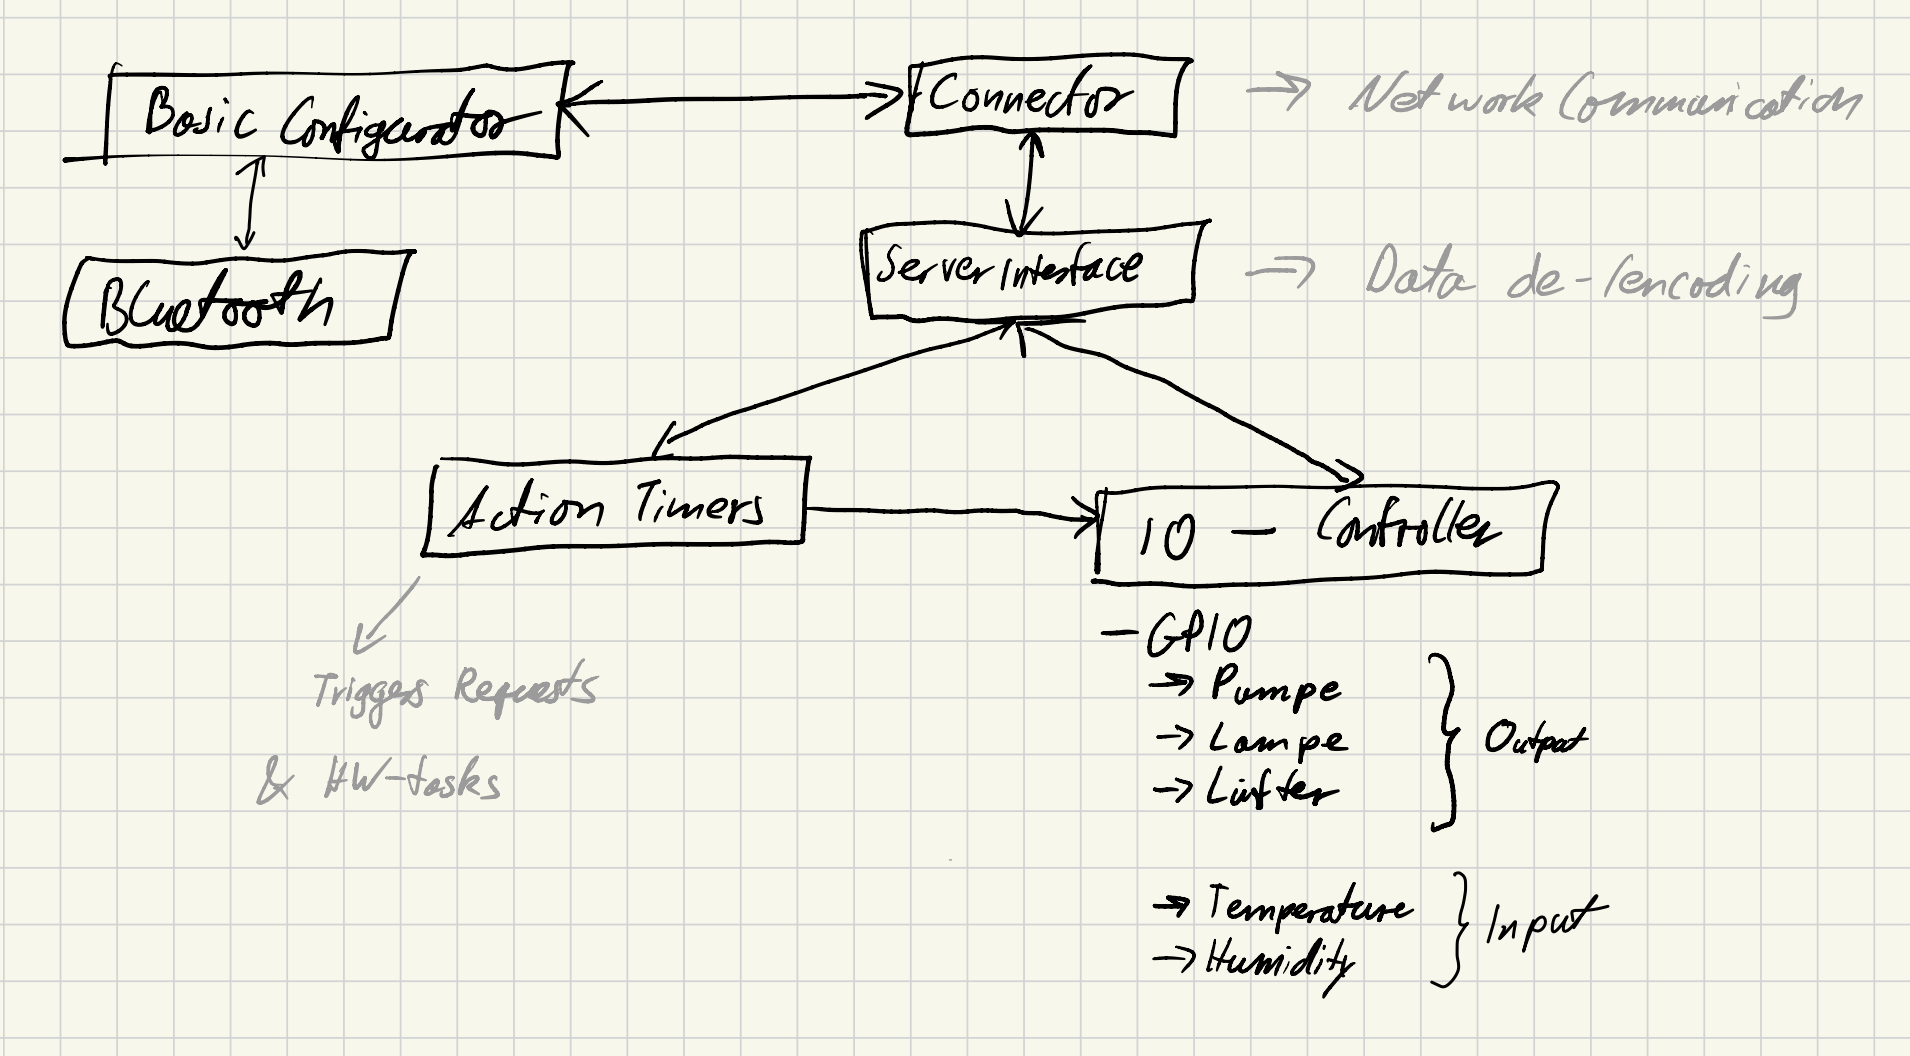
\includegraphics[width=0.8\textwidth]{images/sketch_hardware}
                \caption{Beispielhafte Skizze zur Umsetzung von Hardware-Anforderungen}
                \label{fig:example}
            \end{figure}

            Anhand dieser Zeichnung gelang es komplexe Sachverhalte auf das Wesentliche zu reduzieren und so 
            die Implementierung zu planen. 
            
            
            \item \textbf{Frontend}\\
            Im Frontend wurden beispielsweise Mockups erstellt, um die Änderung am User Interface zu planen. 
            So konnten beispielsweise Proportion von Graphelementen zu Verwaltungsleiste auf der Datenseite der
            Webanwendung modelliert werden. Dadurch wurde die Implementierung erleichtert, da man die Anordnung 
            der Oberflächenelemente nicht in der Entwicklung anpassen muss. Die dafür verwendete Software war 
            Keynote. 

            \item \textbf{Backend}
        \end{itemize}

        \subsubsection*{Implementierung}
            Den erarbeiteten Plan gilt es in dieser Phase eines Zyklus umzusetzen. Die vorherigen 
            Arbeitsabläufe halfen vor allem dabei, die Implementierung zu beschleunigen. Innerhalb dieser Phase 
            wurden ebenfalls in den einzelnen Teams unterschiedliche Verfahren verwendet. Besonders hervorzuheben 
            waren Kanban-Boards, die sowohl im Hardware- und Frontend-Team verwendet. So konnte ein schneller 
            Überblick über die im Team bearbeiteten Themen gewonnen werden. Gerade bei der Implementierung von 
            einzelnen Features half das besonders größere Probleme in kleine handhabbare aufzuteilen. \\
            Da das Backend ausschließlich von Florian erstellt wurde, hat er sich dafür entschieden die anstehenden 
            Aufgaben mittels einer einfachen txt-Datei zu dokumentieren. Das hatte den Vorteil, dass die interne 
            Entwicklung an diesem Teil im Projekt schlank gehalten wurde. \\

        \subsubsection*{Testung}
            Die Testung der implementierten Features im Projekt gilt es im Anschluss zu testen. Die Testung ist ein 
            wesentlicher Bestandteil, der in dem entsprechende Abschnitt näher beleuchtet wird. Aus diesem Grund 
            wird hier nicht mehr näher darauf eingegangen. 

        \subsubsection*{Evaluation}
            In wöchentlichen Meetings während der Software Engineering Vorlesung wurde sich getroffen und frei über das 
            Projekt gesprochen. In diesem Zusammenhang ging es vor allem um den Fortschritt, der in der letzten 
            Woche erzielt wurde und was für die nächste Woche geplant ist. In diesem Zusammenhang konnten die 
            Ergebnisse der einzelnen Entwicklungszyklen hinterfragt werden. Dieses Feedback galt dann entweder der 
            Verbesserung aktueller Ergebnisse oder des nächsten Entwicklungszyklus. \\
            Darüber hinaus galten diese Meetings auch der Kommunikation zwischen den Teams. Bei unserem Automated 
            Greenhouse ist ein wesentlicher Bestandteil die Zusammenarbeit zwischen den Teams im Projekt. Die 
            unterschiedlichen Aufgabenbereiche müssen so aufeinander abgestimmt werden, dass die Teams trotz Differenzen 
            im Fortschritt weiter an ihren Aufgaben arbeiten können. Beispielhaft kann man hier die 
            Endpunkte der API nennen. Diese verbinden das Frontend mit den Sensoren und Aktoren der Hardware und 
            werden von dem Backend implementiert und bereitgestellt. Man erkennt, dass die Entwicklung sehr stark
            voneinander abhängt und deshalb die Meetings sich zu einem sehr wichtigen Bestandteil unseres Vorgehen
            entwickelt haben.

\pagebreak
